\section{Filters}
In ham radio applications it is very important, that transmitted signals are only in the licensed band. This power amplifier works for the 2m band, that means a frequency range of 144MHz to 146MHz.
Of course, also the received signals should be filtered to avoid any unwanted noise.
\subsection{Air Coil Calculation}
The air coils for the TX-OUT and RX-IN filters according to circuit \ref{fig:TX-OUT Filter_Circuit} and \ref{fig:RX-IN Filter_Circuit} can be calculated with the following formula:
\begin{equation}
	L = \frac{N^{2} \cdot d^{2}}{18 \cdot d + 40 \cdot l}
\end{equation}
 Where:
\begin{itemize}
	\item L = Inductance
	\item N = Number of turns
	\item d = Coil outside diameter
	\item l = Length of the coil
\end{itemize}

\bigskip
For a faster result, also an online calculator\footnote{\url{https://m0ukd.com/calculators/air-cored-inductor-calculator/}} \cite{airCoilCalculator.2015} can be used. 

\newpage
\subsection{TX-IN Filter}
This filter is build up with SMT components because of the low input power of 0.5W.
The TX-IN filter is a seventh order chebyshev low pass filter with a cutoff frequency of 175MHz.
The high order is chosen because of the high harmonic distortion of the DRA818V \acs{TRX} at the input.
\begin{figure}[ht!]
	\centering
	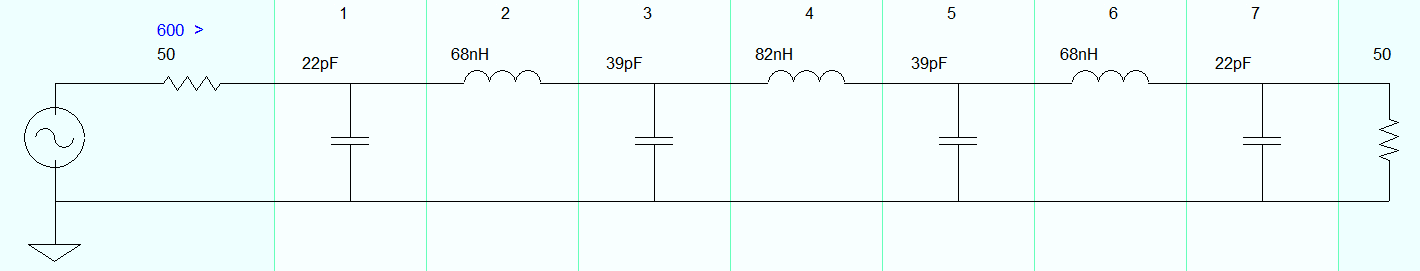
\includegraphics[width = 17cm]{./2_circuit/fig/TX-IN Filter_Circuit}
	\caption{Circuit of the TX-IN Filter}
	\label{fig:TX-IN Filter_Circuit}
\end{figure}
\bigskip
\begin{figure}[ht!]
	\centering
	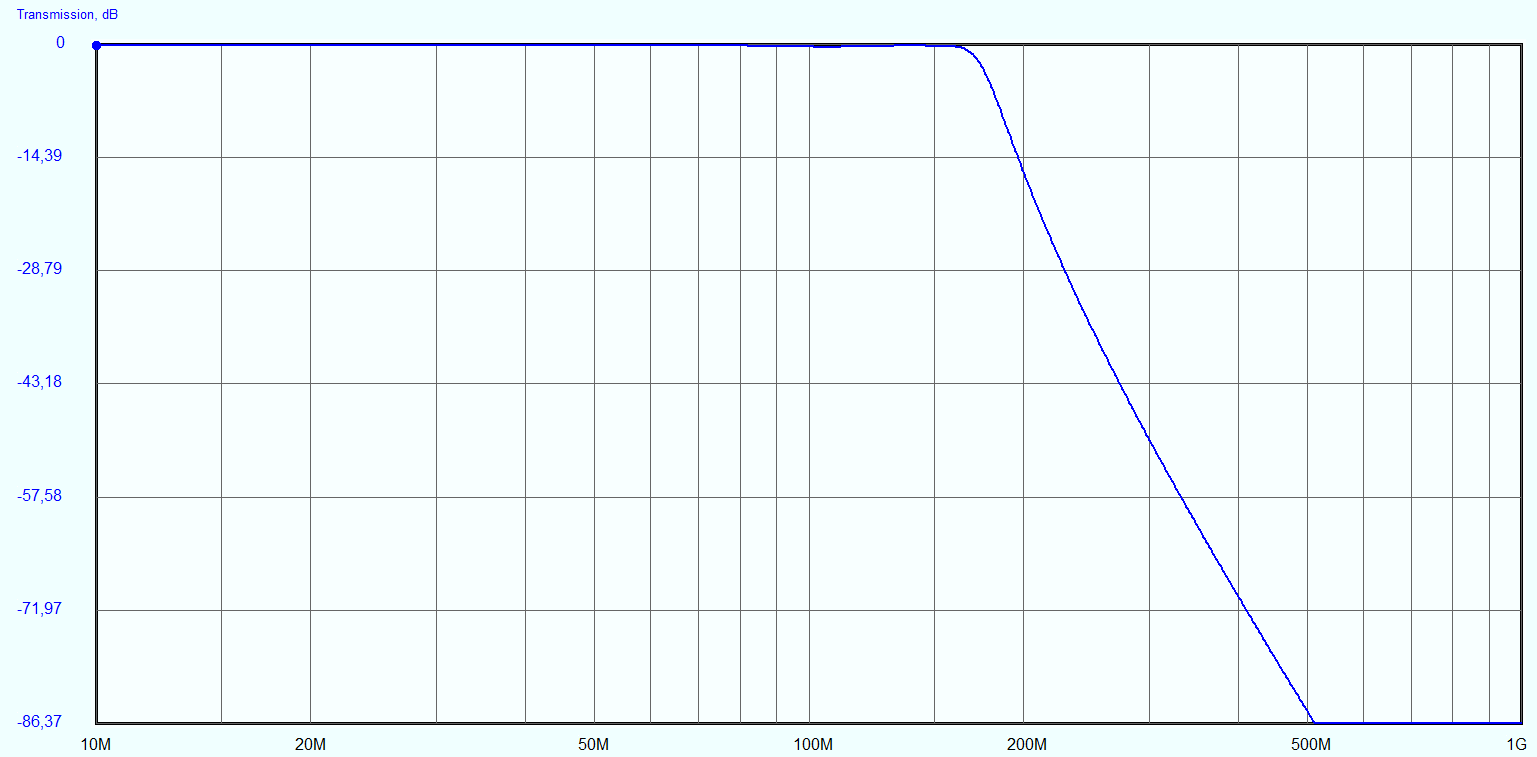
\includegraphics[width = 17cm]{./2_circuit/fig/TX-IN Filter_TF}
	\caption{Transfer Function of the TX-IN Filter}
	\label{fig:TX-IN Filter_TF}
\end{figure}

\newpage
\subsection{TX-OUT Filter}
This filter is build up with self-wound inductors because of the higher output power of 60W.
The TX-OUT filter is a fifth order chebyshev low pass filter with a cutoff frequency of 182MHz.

\begin{figure}[ht!]
	\centering
	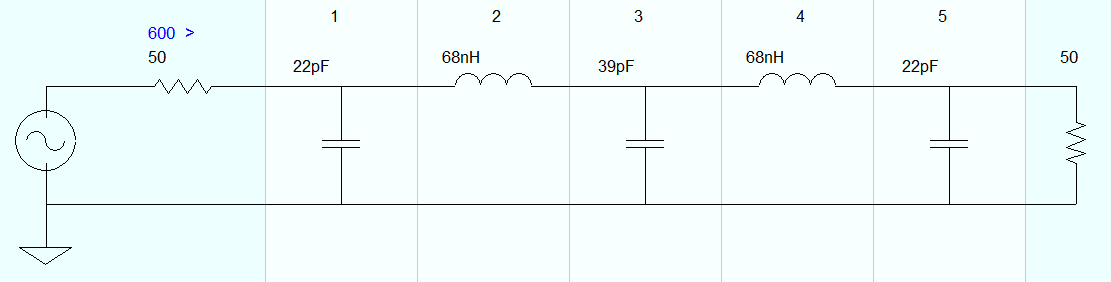
\includegraphics[width = 17cm]{./2_circuit/fig/TX-OUT Filter_Circuit}
	\caption{Circuit of the TX-OUT Filter}
	\label{fig:TX-OUT Filter_Circuit}
\end{figure}
\bigskip
\begin{figure}[ht!]
	\centering
	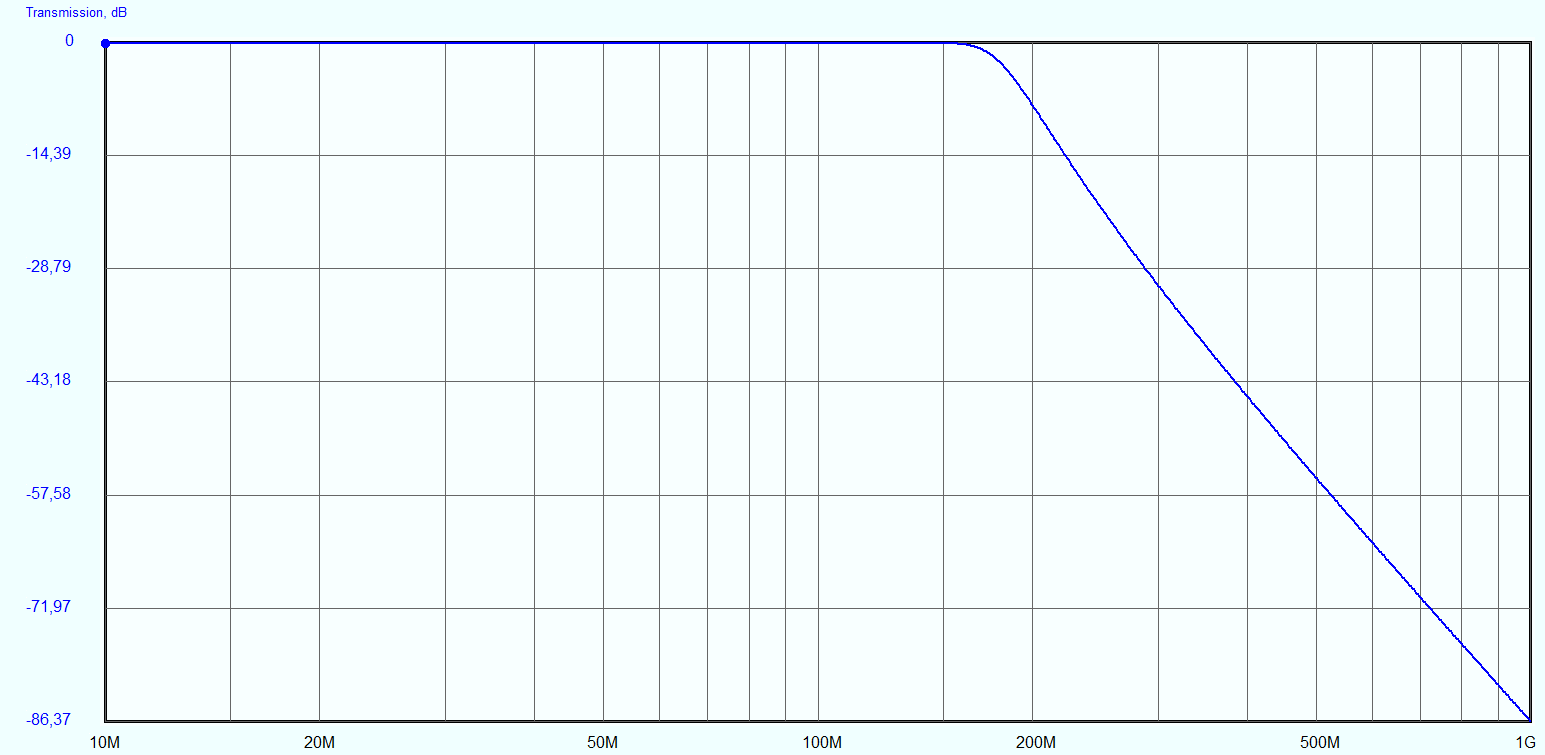
\includegraphics[width = 17cm]{./2_circuit/fig/TX-OUT Filter_TF}
	\caption{Transfer Function of the TX-OUT Filter}
	\label{fig:TX-OUT Filter_TF}
\end{figure}

\newpage
\subsection{RX-IN Filter}
This filter can be build up with SMT components. However, self-wound inductors can be changed easier and the filter band can be adjusted slightly.
The RX-IN filter is a third order chebyshev band pass filter with a lower cutoff frequency of 120MHz and a upper cutoff frequency of 172MHz.

\begin{figure}[ht!]
	\centering
	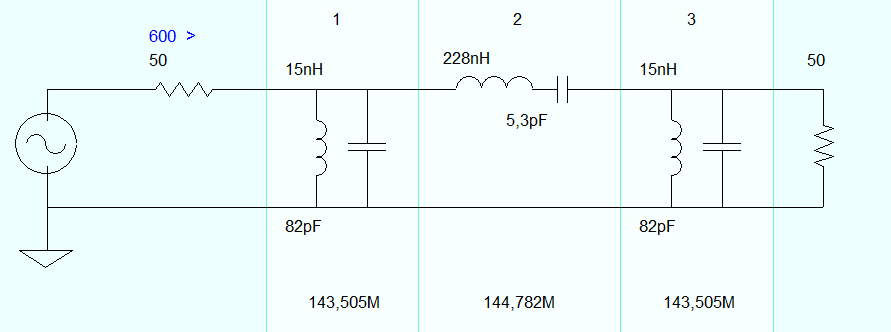
\includegraphics[width = 17cm]{./2_circuit/fig/RX-IN Filter_Circuit}
	\caption{Circuit of the RX-IN Filter}
	\label{fig:RX-IN Filter_Circuit}
\end{figure}
\bigskip
\begin{figure}[ht!]
	\centering
	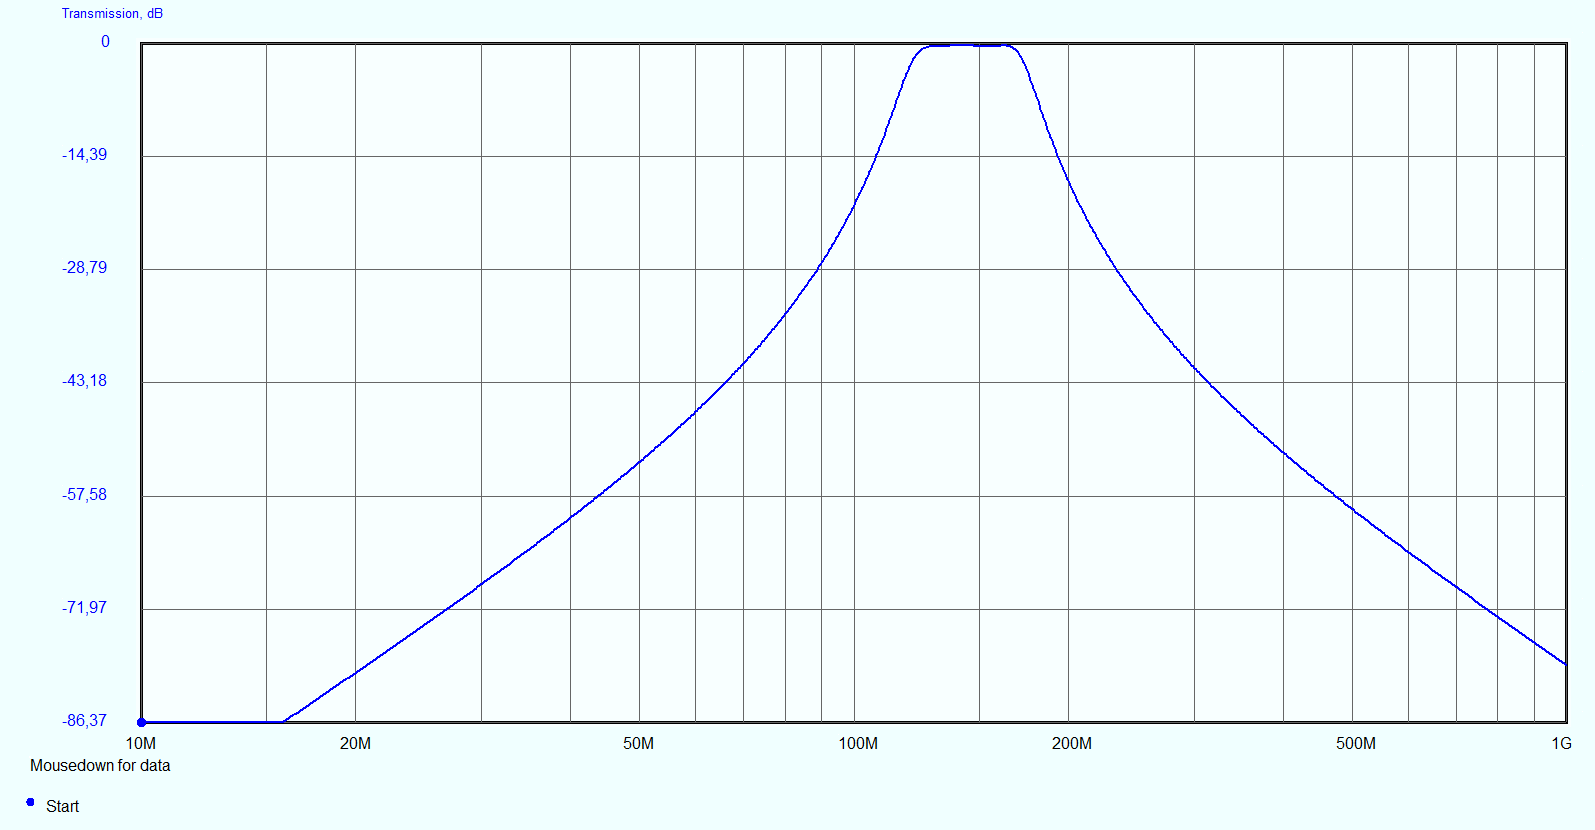
\includegraphics[width = 17cm]{./2_circuit/fig/RX-IN Filter_TF}
	\caption{Transfer Function of the RX-IN Filter}
	\label{fig:RX-IN Filter_TF}
\end{figure}

\newpage
\section{PIN-Diode Switches}
In this project, PIN-Diodes are used instead of relais to switch between RX and TX path.
\subsection{RX/TX Input-Switch}
ToDo Text
\begin{figure}[ht!]
	\centering
	%\includegraphics[width = 12cm]{./2_circuit/fig/}
	\includegraphics[width = 12cm]{example-image}
	\caption{Circuit of the RX/TX Input-Switch}
	\label{fig:RX/TX Input-Switch}
\end{figure}

\newpage
\subsection{RX/TX Output-Switch}
ToDo Text
\begin{figure}[ht!]
	\centering
	%\includegraphics[width = 12cm]{./2_circuit/fig/}
	\includegraphics[width = 12cm]{example-image}
	\caption{Circuit of the RX/TX Output-Switch}
	\label{fig:RX/TX Output-Switch}
\end{figure}